\documentclass[10pt,twocolumn,letterpaper]{article}
\usepackage[10pt,inchmargins]{sigmin}  %% template from Xi Wang.
\special{papersize=8.5in,11in}
\setlength{\pdfpagewidth}{8.5in}
\setlength{\pdfpageheight}{11in}
\usepackage[noheadfoot,
            left=1in,right=1in,top=1in,bottom=1in,
            columnsep=0.3in
            ]{geometry}
\usepackage[small,compact]{titlesec}
\usepackage[font={small,bf}]{caption}    % added 9/10/13
\usepackage[nolineno,noindent,norules]{lgrind}
\usepackage{tightenum}
\usepackage{float}
\usepackage{xspace}
\usepackage{times,pifont}
\usepackage{mathptmx}
\usepackage{subfig,graphics,graphicx,color}
\usepackage{multirow}
\usepackage{dblfloatfix} %% correctly orders single- and double-col figures
\usepackage{hyphenat}
\usepackage{mathrsfs}
\usepackage{subfig}
\usepackage{amssymb,amsmath,centernot}
\usepackage{lastpage}
\usepackage{flushend}
\usepackage{hhline}
\usepackage{authblk}
\newcommand{\doi}{10.1145/2797022.2797033}


%% ================= START of SOSP '13 template ================= 
 \makeatletter
 
 \def\ftype@copyrightbox{8}
 \def\@copyrightspace{
 \@float{copyrightbox}[b]
 \begin{center}
 \setlength{\unitlength}{1pc}
 \begin{picture}(20,6.8) 
 \put(0,3){\parbox{\columnwidth}{\scriptsize
 
 %*** SAMPLE. AUTHOR PUT SUPPLIED TEXT HERE ****
 
 \noindent
 \rule{6.0 cm}{0.2pt}\\
Permission to make digital or hard copies of all or part of this work for personal or classroom use is granted without fee provided that copies are not made or distributed for profit or commercial advantage and that copies bear this notice and the full citation on the first page. Copyrights for components of this work owned by others than ACM must be honored. Abstracting with credit is permitted. To copy otherwise, or republish, to post on servers or to redistribute to lists, requires prior specific permission and/or a fee. Request permissions from Permissions@acm.org.
 
 \vspace{\baselineskip}\noindent
%  Copyright is held by the Owner/Author(s).\\
 \textit{Submitted to APSys '16, August 4-5, 2016, Hong Kong, China}.\\
%  2015 ACM. ISBN 978-1-4503-3554-6/15/07\$15.00. 
%  \noindent
%  http://dx.doi.org/\doi
 }
 }
 \end{picture}
 \end{center}
 \end@float}
 
 \def\maketitle{\par
  \begingroup
    \def\thefootnote{\fnsymbol{footnote}}
    \def\@makefnmark{\hbox
        to 0pt{$^{\@thefnmark}$\hss}}
      \twocolumn[\@maketitle]
 \@thanks
  \endgroup
  \setcounter{footnote}{0}
  \let\maketitle\relax
  \let\@maketitle\relax
  \gdef\@thanks{}\gdef\@author{}\gdef\@title{}\gdef\@subtitle{}\let\thanks\relax
  \@copyrightspace}
 
 \makeatother

%% ================= END of SOSP '13 template ================= 



%\newcommand{\comment}[1]{}
\frenchspacing

%\doublespacing

%%%%%%%%%%%%%%%%%%%%%%%%%%%%
%     macro

\newcommand{\xxx}{\mbox{\textsc{REPVM}}\xspace}
\newcommand{\mytitle}[0]{\textbf {\xxx}}
\newcommand{\mykeywords}[0]{State Machine Replication, High Availability, Virtual Machine,
  Software Reliability}

%%%%%%%%%%%%%%%%%%%%%%%%%%%%%%%%%%%%%%%%%%%%%%%%%%%%%%%%%%%%%%%%%
% hyperref stuff

\usepackage[square,comma,numbers,sort]{natbib}
\usepackage{hypernat}
\usepackage{hyperref}

%% fill in pdf info here
\hypersetup{%
colorlinks=false,
pdfborder={0 0 0},
pdftitle={\mytitle},
pdfkeywords={\mykeywords},
bookmarksnumbered,
pdfstartview={FitH},
urlcolor=cyan,
pdfpagelabels=true,
pdfdisplaydoctitle=true,
}%

%\usepackage{breakurl}
%\usepackage[all]{hypcap}
%\renewcommand{\url}{\burl}

%%%%%%%%%%%%%%%%%%%%%%%%%%%%%%%%%%%%%%%%%%%%%%%%%%%%%%%%%%%%
% Some NICE fonts

\newfont{\BIG}{cminch}                             %--- One-inch font
\newfont{\sfbHuge}{cmssbx10 scaled\magstep5}       %-- 25pt sans serif bold
\newfont{\sfbLarger}{cmssbx10 scaled\magstep3}   %-- 12+pt sans serif boldd
\newfont{\sfblarger}{cmssbx10 scaled\magstep2}   %-- 12+pt sans serif bold
\newfont{\sfblarge}{cmssbx10 scaled\magstep1}      %-- 12pt sans serif bold
\newfont{\sfbeleven}{cmssbx10 scaled\magstephalf}  %-- 11pt sans serif bold
\newfont{\sfb}{cmssbx10}                           %-- 10pt sans serif bold
\newfont{\sfeight}{cmss8}                          %-- 8pt sans serif

%%%%%%%%%%%%%%%%%%%%%%%%
%    space tweaking

%\textwidth = 6.5 in
%\textheight = 9.0 in
%\setlength{\topmargin}{-.5in}

%\headheight = 0.0 in
%\headsep = 0.0 in
%\parskip = 0.2in
%\parindent = 0.0in

\renewcommand{\topfraction}{0.95}
\addtolength{\textfloatsep}{-0.1in}
%\addtolength{\floatsep}{0.025in}
\renewcommand\floatpagefraction{.9}
%\renewcommand\bottomfraction{.9}
\renewcommand\textfraction{.1}

\setlength{\parindent}{9pt}

% Rescue
\makeatletter
\def\v#1{{\mbox{\fontfamily{cmtt}\fontsize{\f@size}{\f@size}\selectfont #1}}}

\newcommand{\smt}[0]{StableMT\xspace}
\newcommand{\smr}[0]{SMR\xspace}
%\newcommand{\tsmr}[0]{TSMR\xspace}

\newcommand{\us}[0]{\(\mu\text{s}\)\xspace}
\newcommand{\ms}[0]{ms\xspace}
\newcommand{\paxos}[0]{\textsc{Paxos}\xspace}
\newcommand{\calvin}[0]{\textsc{Calvin}\xspace}
\newcommand{\repbox}{\mbox{\textsc{Crane}}\xspace}
\newcommand{\protocol}{\mbox{\textsc{DARE}}\xspace}
\newcommand{\racepro}[0]{\textsc{RacePro}\xspace}
\newcommand{\criu}[0]{\textsc{CRIU}\xspace}
\newcommand{\peregrine}[0]{\textsc{Peregrine}\xspace}
\newcommand{\grace}[0]{Grace\xspace}
\newcommand{\coredet}[0]{\textsc{CoreDet}\xspace}
\newcommand{\kendo}[0]{Kendo\xspace}
\newcommand{\dos}[0]{dOS\xspace}
\newcommand{\ddos}[0]{DDOS\xspace}
\newcommand{\ldpreload}[0]{LD\_PRELOAD\xspace}

\newcommand{\apache}{\v{Apache}\xspace}
\newcommand{\mongoose}[0]{\v{Mongoose}\xspace}
\newcommand{\ab}{\v{ApacheBench}\xspace}
\newcommand{\clamav}{\v{ClamAV}\xspace}
\newcommand{\clamdscan}{\v{clamdscan}\xspace}
\newcommand{\upnp}{uPnP\xspace}
\newcommand{\mediatomb}{\v{MediaTomb}\xspace}
\newcommand{\mencoder}{\v{mencoder}\xspace}
\newcommand{\mongodb}{\v{MongoDB}\xspace}
\newcommand{\ssdb}{\v{SSDB}\xspace}
\newcommand{\mysql}{\v{MySQL}\xspace}
\newcommand{\sysbench}{\v{SysBench}\xspace}
\newcommand{\zookeeper}{\v{ZooKeeper}\xspace}


\newcommand{\aget}[0]{\v{aget}\xspace}
\newcommand{\pthread}[0]{\mbox{Pthreads}\xspace}
\newcommand{\openldap}[0]{{OpenLDAP}\xspace}
\newcommand{\redis}[0]{{Redis}\xspace}
\newcommand{\bdb}[0]{{Berkeley DB}\xspace}
\newcommand{\vtune}[0]{\v{VTune}\xspace}
\newcommand{\http}[0]{\mbox{HTTP}\xspace}

% In short.
\newcommand{\eg}{{e.g.}}
\newcommand{\ie}{{i.e.}}
\newcommand{\etc}{{etc}}
\newcommand{\para}[1]{\vspace{.00in}\noindent{\bf #1}}
\newcommand{\wrt}{{w.r.t. }}
\newcommand{\cf}{{cf. }}

% Synch and network operations.
\newcommand{\mutexlock}[0]{\v{pthread\_mutex\_lock()}\xspace}
\newcommand{\connect}[0]{\v{connect()}\xspace}
\newcommand{\send}[0]{\v{send()}\xspace}
\newcommand{\close}[0]{\v{close()}\xspace}
\newcommand{\recv}[0]{\v{recv()}\xspace}
\newcommand{\select}[0]{\v{select()}\xspace}
\newcommand{\poll}[0]{\v{poll()}\xspace}
\newcommand{\epollwait}[0]{\v{epoll\_wait()}\xspace}
\newcommand{\accept}[0]{\v{accept()}\xspace}
\newcommand{\tapsend}[0]{\v{tap\_send()}\xspace}
\newcommand{\taprecv}[0]{\v{tap\_receive()}\xspace}

% Parrot primitives.
\newcommand{\getturn}[0]{\v{get\_turn()}\xspace}
\newcommand{\putturn}[0]{\v{put\_turn()}\xspace}
\newcommand{\wait}[0]{\v{wait()}\xspace}
\newcommand{\signal}[0]{\v{signal()}\xspace}

% Evaluation stats.
\newcommand{\github}[0]{\url{anonymous}}
\newcommand{\ntype}[0]{three\xspace}
\newcommand{\nprog}[0]{four\xspace}
\newcommand{\overhead}[0]{1.8\%\xspace}
\newcommand{\dmtspeedup}[0]{10.5\%\xspace}
\newcommand{\proxyoverhead}[0]{1.7\%\xspace}
\newcommand{\recovertime}[0]{0.82s\xspace}
\newcommand{\mencoderspeedup}{\v{49\%}\xspace}

\newcommand{\tputoverhead}[0]{3.22\%\xspace}
\newcommand{\latencyoverhead}[0]{3.31\%\xspace}

\def\LGfsize{\footnotesize}
%\pagestyle{empty}

\begin{document}

% Hack for: Package caption Error: No float type 'copyrightbox' defined.
%\newcounter{copyrightbox}

\date{}

\title{\mytitle}

% \author[+*]{\hspace{0 mm}\fontsize{10}{10}\selectfont Heming Cui}
\author{Paper \#10}
% \author[*]{Cheng Liu}
% \author[*]{Junfeng Yang}
% \setlength{\affilsep}{1em}
% \renewcommand\AB@affilsepx{\hspace{28.0 mm}\protect\Affilfont}
%\affil[+]{Department of Computer Science}
%\renewcommand\AB@affilsepx{\\\protect\Affilfont}
%\affil[*]{Department of Computer Science\hspace{1.0mm}}
% \affil[+]{\textrm\fontsize{10}{10}\selectfont The University of Hong Kong}
% \affil[*]{\textrm Columbia University\vspace{-7.0 mm}}


\maketitle
%\thispagestyle{empty}

\begin{sloppypar}
\begin{abstract}
% The fault tolerance and the theoretically proven safety of state machine
% replication (\smr) makes it attractive for implementing a principled
% system for general programs, especially server programs that demand high
% availability.  Unfortunately, existing \smr systems unrealistically assume
% deterministic code execution when most server programs are
% nondeterministic multithreaded programs.  Moreover, existing \smr systems
% typically provide narrow state machine interfaces, and orchestrating a
% sever program into these interfaces can be strenuous and error-prone.
% 
% This paper presents \xxx, an \smr system that transparently replicates
% general server programs for high availability.  It interposes on the
% socket and the thread synchronization interfaces to keep replicas in sync
% for transparency, requiring no intrusive modifications to shoehorn a
% program into a narrow interface.  To address nondeterminism, \xxx
% leverages deterministic multithreading to keep replicas in sync.  \xxx
% addresses a difficult network input timing problem via a new technique
% called \emph{time bubbling}. Evaluation on three diverse types of four
% widely used server programs (\eg, \apache and \clamav) show that \xxx is
% easy to use, has reasonable overhead (\overhead in average), and is robust.

Dynamic program analysis frameworks have become increasingly pervasive and 
critical because they enable a wide range of powerful analysis tools (\eg, 
reliability, profling, and logging) at runtime to improve the quality of 
software applications. An open problem for existing frameworks is 
performance: to analyze an application's execution, these frameworks frequently 
synchronize execution states (\eg, accessed memory and thread interleavings) 
between the actual execution and the analysis, causing prohibitive slowdown in 
the execution. To reduce synchronizaing execution states, many frameworks 
require significantly reconstructing analysis tools as well as the frameworks 
themselves, which heavily trades off transparency between the analysis and the 
framework and allows only one analysis to be run at the same time.


This paper presents \xxx, an efficient and transparent framework by leveraging 
two techniques: state machine replication (SMR) and deterministic 
multithreading (DMT). SMR ensures that replicas running the same application 
always see the same sequence of inputs, then multiple analyses can run within 
some replicas transparently. DMT efficiently enforces the same thread 
interleavings across replicas and eliminates the need of synchronizing 
schedules between execution and analysis. Evaluation shows that \xxx is easy to 
plug in analysis tools and has reasonable overhead.
\end{abstract}
\end{sloppypar}

% \begin{sloppypar}
%% %\category{D.2.5}{Software Engineering}{Testing and Debugging}
%% \category{D.4.5}{Operating Systems}{Threads, Reliability}
%% \category{D.2.4}{Software Engineering}{Software/Program Verification}
%% \terms{Algorithms, Design, Reliability, Performance}
%% \keywords{\mykeywords}

%% \vskip 2mm
%% \noindent {\small \bf Categories and Subject Descriptors:} \vskip -.2mm
%% \noindent
%% {\footnotesize D.4.5~[{\bf Operating Systems}]: {Threads, Reliability}\\
%% D.2.4~[{\bf Software Engineering}]: {Software/Program Verification};}
%% \vskip 1mm
%% \noindent {\small \bf General Terms:} \vskip -.2mm
%% \noindent
%% {\footnotesize Algorithms, Design, Reliability, Performance}
%% \vskip 1mm
%% \noindent {\small \bf Keywords:} \vskip -.2mm
%% \noindent
%% {\footnotesize \mykeywords}

% \vskip 2mm
% \noindent {\small \bf Categories and Subject Descriptors:}
% {\small D.4.5~[{\bf Operating Systems}]: {Threads, Reliability};
%   D.2.4~[{\bf Software Engineering}]: {Software/Program Verification};}
% \vskip .1mm
% \noindent {\small \bf General Terms:} {\small Algorithms, Design,
%   Reliability, Performance}
% \vskip .1mm
% \noindent {\small \bf Keywords:} {\small \mykeywords}
% 
% \end{sloppypar}

%%%%%%%%%%%%%%%%%%%%%%%%%%%%%%%%%%%
% Add page number.
\setcounter{page}{1}
\pagenumbering{arabic}

\thispagestyle{plain}
\pagestyle{plain}
\setlength{\footskip}{20pt}
%%%%%%%%%%%%%%%%%%%%%%%%%%%%%%%%%%%

\begin{sloppypar}

\section{Introduction} \label{sec:intro}

% P1: lots of applications require various big data frameworks. Trading, fraud 
% detection, aviation, medical, military. But existing systems can not meet the 
% high latency and availability requriements of these applications.
Driven the the drastically increasing computational demands and the volumns of 
data, more and more applications are being pushed to deploy in cluster 
managemement systems~\cite{mesos,borg,helix,yarn} in order to harness the 
computational resources in clusters. These applications not only include typical 
big-data frameworks (\eg,~\cite{spark}), but also critical applications such as 
trading platforms, fraud detection systems, health care systems, and military 
systems. We consider an application \emph{critical} if its high requirements on 
availability and response time. For example, a high-frequency trading platform 
tends to be highly-availabile during the stock operation hours, and adding a 
few hundred \us to the platform's response time means huge money lost.

Unfortunately, despite recent advances in building and applying cluster 
managemement systems~\cite{mesos,borg,helix,yarn}, these systems are still 
difficult to meet the high requirements of critical applications because these 
systems do not provide high-availability to the applications. Specifically, to 
make the systems themselves highly-availabile, existing systems typically 
replicate their controller component which accepts tasks, allocate 
computational resources, and (re)schedule tasks on availabile resources. 
However, the applications themselves are not replicated: if an application 
crashes or a computational resource goes down (\eg, hardware errors), these 
systems have to reschedule the tasks, leaving an arbitral unavailable time 
window for these applications. A possible key reason of this problem is that 
these systems are initially designed for big-data engines which already 
considered fault recovery (but, not availability).

% P2: SMR a promising approach, but slow.
State machine replication (SMR)~\cite{paxos} may be a promising approach 
to address the availability problem of critical applications. SMR runs the 
same program on a number of replicas and uses a distributed consensus protocol 
(\eg, 
\paxos~\cite{paxos:practical,paxos,paxos:simple,paxos:complex,epaxos:sosp13}) 
to enforce the same inputs among 
replicas. Typically, \paxos assigns a replica as the leader to propose 
consensus requests, and the other replicas agree or reject requests. 
An input consensus can achieve as long as a majority of replicas 
agree, thus SMR can tolerate various faults such as minor replica failures. For 
instance, two existing systems \borg~\cite{borg} and \mesos~\cite{borg} use 
\paxos to replicate their controllers.

However, \paxos's consensus is notoriously difficult to be fast. 
To agree on an input, traditional consensus protocols invoke at least one 
message round-trip between two replicas. Given that a \v{ping} in Ethernet 
takes hundreds of \us, a program running in an SMR system with three replicas 
must wait at least this time before processing an input. 

% P3: RDMA, new opportunity. Two RDMA systems.
Remote Direct Access Memory (RDMA) is a promising technique to mitigate 
consensus latency because recently it becomes cheaper and increasingly 
pervasive in datacenters. RDMA allows a process to directly write to the 
user space memory of a remote process, completely bypassing the remote OS 
kernel or CPU (the so called ``one-sided" operations). An 
evaluation~\cite{pilaf:usenix14} shows that such a write round-trip takes only 
$\sim$3 \us in the Infiniband architecture~\cite{infiniband}. Two recent 
RDMA-enabled \paxos implementations~\cite{dare:hpdc15,falcon:github} reported 
$\sim$15 \us consensus latency.

% As a common 
% RDMA practice, to ensure that such a write successfully resides in the 
% memory of a remote process, the local process should wait until the remote NIC 
% (network interface card) sends an ACK to the local host's NIC. 

% P4: We present a new fast, highly-available computing platform by building a 
% eco system with Mesos and RDMA SMR systems.

% Benefits.

% P5: Applications enjoy better latency and fault-tolerance.

% P6: Benefit, now frameworks can focus on their own logic, no longer need 
% fault-toelrance module. Fault-tolerance requires expert knowledge, really 
% hard to build.

% P7: Can also address the performance problem: slow tail.

% P8: in essense, a datacenter OS: handles resource allocation/isolation, 
% fault-tolerance, and performance for frameworks (applications). Use 
% replication to bstract away % physical machine details; frameworks now only 
% see computing resources, safely ignore other things such as physical 
% machines, fault-tolerance, and tails.

% P9: Feasibility study.

% P10: rest of the paper.



\section{Background} \label{sec:background}

\subsection{KVM} \label{sec:kvm}

KVM is a more recent hypervisor which embeds virtualization capabilities 
in Linux kernel using x86 hardware virtualization extensions~\cite{kivity2007kvm}. 
It is a full virtualization solution, where guests are run unmodified in VMs. It 
consists of two modules, namely, kvm.ko module and an architecture dependent 
kvm-amd.ko or kvm-intel.ko module. Under KVM, each VM is spawned as a regular linux 
process named KVM and scheduled by the default linux scheduler. 

For using shared I/O hardware, these VMs interact with Qemu emulator in host user 
space which provides emulated I/O devices for virtual machines. For instance, in 
the case of network related applications, Qemu provides emulated Network Interface 
Card (NIC) to VMs and interacts with tun-tap device on the other side. The tap device 
is connected to physical NIC through a software bridge.

Figure 1 shows the typical KVM architecture, with reference to a network related
application. 

As depicted in the picture, when a packet arrives at physical NIC,
interrupts generated by NIC are handled by the physical device driver. The device
driver forwards the packet to software bridge. The bridge, then pushes the packet
to the tap device of the corresponding VM. The tap device is a virtual network
device that sends a signal to KVM module. KVM module in turn, generates a virtual
interrupt to the user space Qemu of the target VM. Qemu then copies the packet from
tap device and generates the interrupt for the guest OS emulating the virtual NIC.
Again, the physical device driver in the guest OS handles the packet transfer to
the VM’s address space. A major advantage of the KVM architecture is the full
availability of user-space tools in the QEMU process, such as threading, libraries
and so on.

\begin{figure}[t]
% \vspace{.20in}
\centering
\includegraphics[width=.47\textwidth]{figures/kvm}
\vspace{-.2in}
\caption{{\em KVM Architecture.}} \label{fig:kvm}
\vspace{.05in}
\end{figure}

\subsection{FALCON} \label{sec:falcon}

\smrsystem's deployment model is similar to a typical \smr's. In a \smrsystem-replicated 
system, a set of $2f+1$ machines (nodes) are set up in a InfiniBand cluster. Once the 
\smrsystem system starts, one node becomes the \emph{primary} node which proposes the order of 
requests to execute, and the others become backup nodes which follow the primary’s 
proposals. An arbitrary number of clients in LAN or WAN send network requests to the 
primary and get responses. If failures occur, the nodes run a leader election to elect 
a new leader and continue.

On receiving a client network request, it invokes a RDMA-based consensus process on this 
request to enforce that all replicas see the same sequence of input requests. This process 
has three steps. In the first step, the leader assigns a global, monotonically increasing 
viewstamp to this request, stores this request into an entry that is appended to the consensus 
log, and does a forced write to the local disk. The second step is to replicate the log entry 
on remote servers using a one-sided RDMA Write operation. Usually when the RDMA NIC (RNIC) 
completes the netwrok steps associated with the RDMA operation, it pushes a completion event 
to the queue pair's associated completion queue (CQ) via a DMA write. Using completion events 
adds extra overhead. Since \paxos could help handle the reliability issues, \smrsystem takes 
advantage of unsignaled RDMA write operations, i.e., a completion event will not be pushed for 
these operations, to reduce that overhead. In the last step, the leader thread waits for 
acknowledgments from a majority of nodes.

In addition to the distributed consensus protocol for coordinating the sequence of input requests, 
\smrsystem also runs an output checking protocol which compares each replica's network outputs 
occasionally to detect the divergence of execution states.

\section{\xxx Overview} \label{sec:overview}

\subsection{Architecture} \label{sec:arch}

Figure 2 shows \xxx's architecture. It contains three main components.

% On receiving a packet, QEMU calls tap_send()
% On sending a packet, QEMU calls tap_receive()

The replication logic is entirely implemented in qemu-kvm, a KVM tailored version of QEMU.
We maintain a packet queue to capture outgoing packets.

\begin{figure}[t]
% \vspace{.20in}
\centering
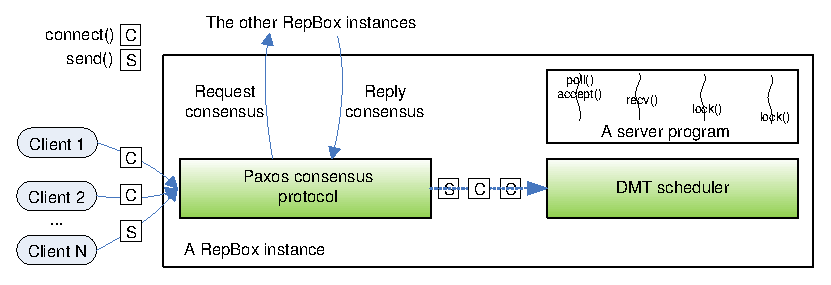
\includegraphics[width=.47\textwidth]{figures/arch}
\vspace{-.2in}
\caption{{\em The \xxx Architecture.}} \label{fig:arc}
\vspace{.05in}
\end{figure}

% \newpage
\section{Evaluation} \label{sec:eval}

% We evaluated an anti-virus scanning server that a b c d e f.

\begin{table}[b]
\footnotesize
\centering
\vspace{-.05in}
\begin{tabular}{lrrr}
{\bf Approach} & {\bf Execution time (ms)} \\
\hline\\[-2.3ex]
Native execution                       & 991        \\
\xxx bare framework only                       & 992        \\
\xxx with Helgrind                                   & 1,048     \\
\xxx with drcov                                   & 1,036     \\
\xxx with Helgrind and drcov                       & 1,012        \\
Helgrind only                       & 41,018       \\
drcov only                       & 1,272       \\
\end{tabular}
\vspace{-.05in}
\caption{{\em \clamav's performance running in \xxx.}}
\label{tab:overhead}
\end{table}

We evaluated \xxx on \clamav~\cite{clamav}, a popular anti-virus scanning 
server that scans files in parallel and deletes malicious ones. Our evaluation was done on a set of three 
Linux 3.2.14 machines within a 1Gbps bandwidth LAN, and each machine has 2.80 
GHz dual-socket hex-core Intel Xeon with 24 hyper-threading cores and 64GB 
memory. To evaluate performance, we used \clamav's own client utility 
\v{clamdscan} to request the \clamav server to spawn 8 threads to scan its own source code 
and installation directories in parallel and measure the utility's execution time. To mitigate network 
latency, the benchmark clients were ran within the LAN. We selected two popular 
analysis tools: one heavyweight tool, the Helgrind race 
detector~\cite{valgrind:pldi}; and one lightweight 
tool, DynamoRio's code coverage tool drcov~\cite{dynamorio}.

Table~\ref{tab:overhead} shows the performance results running \clamav in 
\xxx. \xxx's bare replication framework without any analysis, incorporates 
negligible overhead compared the native execution. The performance overhead of 
running Helgrind only in one replica incurred 5.8\% overhead compared to the native execution, 
because the other replica node and the primary run the native executions and 
reach consensus fast. When running the drcov tool only or running two tools, 
\xxx incurred only 2.1\% to 3.6\% overhead, because the drcov tool incurred 
moderate overhead (28.3\% compared to native execution), and once the drcov 
tool reaches consensus with the primary on the \v{clamdscan} utility's request, 
the primary processes the request and responses fast.

When running Helgrind only with \clamav, the performance slowdown is 40.4X. This result reflects that \xxx's 
replication architecture masks the huge performance slowdown of Helgrind, so 
that client programs feel that \clamav runs efficiently even with the 
powerful analysis turned on. Note that Helgrind is already carried in Valgrind, 
a traditional analysis framework that takes the ``fully-coupled" approach. So 
does drcov for the DynamoRio analysis framework. Overall, this evaluation shows that \xxx is efficient, transparent to the 
Helgrind and drcov, and complementary to an traditional analysis framework 
Valgrind and DynamoRio. in addition, to the best of our knowledge, this 
evaluation is the first one to show that multiple types of analysis tools can 
run together within the same execution.

\section{Related Work} \label{sec:related}

Existing analysis frameworks can be classified into two approaches depending 
on how a framework exposes an application's actual execution states to an 
analysis tool. The first approach in-lines an analysis within an 
actual execution~\cite{dynamorio, pin:pldi05, 
valgrind:pldi, lift:micro06, tsan}, which may cause prohibitive slowdown in the
executions when an analysis does heavyweight work. Recently, researchers have
proposed to 
decouple analysis from execution~\cite{decouple:usenix08, speck:asplos08, 
shadowreplica:ccs13, wester:parallelizing:asplos13, superpin, jungwoo:oopsla09} 
via executing analyses in parallel, record-replay, and so on. We classify these
frameworks into ``partially-decoupled" approach because they still need to
frequently 
transfer execution states from the execution (\eg, effective memory addresses 
and thread interleavings) to analysis. These ``partially-decoupled" frameworks 
have shown 4X$\sim$8X speedup over the traditional frameworks on the same 
analysis, which shows that decoupling analysis from execution is a promising 
direction. \xxx fully decouples analysis from execution via replicating 
equivalent executions.

\smr has been studied by the literature for decades, and it is recognized by 
both industry and academia as a powerful fault-tolerance technique in clouds 
and distributed systems~\cite{lamportclock, smr:tutorial}. As a common 
standard, SMR uses \paxos~\cite{paxos} as the consensus protocol to ensure that 
all nodes see the same input request sequence. In this standard, nodes first 
``agree" on a total order of input request as a input sequence, and then 
``execute" the requests that have reached this consensus. This typical SMR 
approach is called ``agree-execute". SMR systems, including 
Chubby~\cite{chubby:osdi}, ZooKeeper~\cite{zookeeper}, and 
the Microsoft \paxos~\cite{paxos} implementation, have been widely used to 
maintain critical distributed systems configurations (\eg, group leaders, 
distributed locks, and storage meta data). SMR has also been applied broadly to 
build various highly available services, including 
storage~\cite{paxos:datastore} and wide-area network~\cite{mencius:osdi08}. 
Hypervisor-based Fault Tolerance~\cite{hft:sosp95} leverages a hypervisor to 
build a primary-back system for single-core machines. These systems focus on 
specific types of applications (\eg, distributed lock 
service~\cite{chubby:osdi}, file system~\cite{zookeeper}) and thus they are not 
designed to be transparent to general multithreaded applications.

In order to support multithreading in SMR, Eve~\cite{eve:osdi12} introduces a 
new ``execute-verify" approach: it first executes a batch of requests 
speculatively, and then verifies whether these requests have conflicts (\eg, 
different thread interleavings) that cause execution state divergence. If 
conflicts occur, Eve rolls back. Eve's execution divergence verification 
requires developers to manually annotate all shared states in application code, 
thus it is not transparent to applications.

Rex~\cite{rex:eurosys14} addresses the thread interleaving divergence problem 
with a ``execute-agree-follow" approach: it first records thread interleavings 
on the primary node by executing requests, and then replays these interleavings 
on the other backups. Rex requires frequently shipping thread interleavings 
across nodes, which may be slow. Furthermore, Rex requires application 
developers to build their own checkpoint-restore mechanism, thus this mechanism 
is not transparent to applications.

% \repbox~\cite{repbox:sosp15} is the first \smr system that transparently 
% replicates server applications via its socket-API based \paxos consensus 
% interface. Unlike \repbox, \xxx's main purpose is not fault-tolerance. \xxx is 
% a program analysis framework which leverages \repbox's \paxos implementation to 
% transparently support analysis tools. \xxx's main contribution is that it 
% applied the \smr concept to a new domain: constructing multiple equivalent 
% executions to enable efficient and transparent analyses.


\section{Conclusion} \label{sec:conclusion}

TBD.
\end{sloppypar}

% uncomment to tweak with bib spacing
%\setlength\bibsep{2.25pt}
{
%\small
 \bibliographystyle{abbrv}
 \bibliography{bib/biblio}
}

\end{document}
